\ifdefined\XeTeXrevision\else\pdfoutput=1\fi
\documentclass[10pt]{article}
\usepackage[margin=0.82in]{geometry}
\usepackage{amsmath}
\usepackage{amssymb}
\usepackage{booktabs}
\usepackage{graphicx}
\usepackage{microtype}
\usepackage{tabularx}
\usepackage{xcolor}
\usepackage{hyperref}
\hypersetup{
  colorlinks=true,
  linkcolor=blue!55!black,
  citecolor=blue!55!black,
  urlcolor=blue!55!black,
  pdftitle={Eight Soft Tokens Can Change a Frozen Model's Tone},
  pdfauthor={Franci Penov},
}
\graphicspath{{../reproductions/causal-expression/results/qwen36-35b-confirmatory-20260725/figures/}}
\newcommand{\model}{Qwen3.6-35B-A3B}
\newcommand{\code}[1]{\texttt{#1}}
\title{Eight Soft Tokens Can Change a Frozen Model's Tone}
\author{Franci Penov \\ kortexa.ai \\ \texttt{francip@kortexa.ai}}
\date{2026-07-25}

\begin{document}
\maketitle

\begin{abstract}
We test whether a small hidden input can control the interpersonal style of a
frozen language model's complete response. The model is
\model, a mixture-of-experts model with 35B total and 3B active parameters.
For each of three signed social-style axes, we train eight continuous input
embeddings while freezing every model parameter. Training uses content-matched
positive and negative responses to 18 request-axis pairs built from six
synthetic technical requests. Evaluation uses eight held-out requests, three
fresh seeds, greedy decoding, visible style instructions, no-prefix responses,
and wrong-axis controls. The axis-specific writer passes its frozen warmth
rule. Its median generated span is 71.4\% of the span caused by visible style
instructions, and all 24 held-out comparisons have the intended sign and beat
the wrong-axis shift. The score shift is visible in the prose. Two
negative-prefix seeds answer insults, praise, and gratitude with open hostility,
while the third tends to refuse. A shared-center extension raises patience from
15.6\% to 19.5\% of the explicit span, missing its 20\% rule, and its nominal
neutral center drifts on every axis. Eight soft tokens can therefore provide a
causal style writer, but the learned geometry is neither smooth nor reliably
neutral.
\end{abstract}

\section{Introduction}

A persistent social state needs a writer that changes what a model says. A
state that moves in an internal probe while decoded responses remain unchanged
has no demonstrated expression channel. This paper isolates that writer. It
does not train a session reader, update state from conversation history, or
apply temporal decay.

Soft prompt tuning learns input embeddings while holding the language model
fixed \cite{lester2021prompt}. Prefix tuning extends the idea with continuous
activations available throughout generation \cite{li2021prefix}. Activation
steering instead adds learned directions inside the model during a forward
pass; contrastive activation addition has changed open-ended behavior in
Llama~2 \cite{rimsky2024caa}. Our intervention stays at the input embedding
layer. An oracle coordinate selects eight learned soft tokens immediately
before the assistant header.

The evaluation measures complete-response direction, wrong-axis specificity,
and the neutrality of a shared center. Warmth passes the first two tests. The
shared-center result is negative.

\section{Method}

\subsection{Frozen model and learned prefixes}

We use the post-trained \model\ checkpoint at revision
\code{995ad96eacd98c81ed38be0c5b274b04031597b0}. The model card reports 35B
total parameters, 3B active parameters, a 2,048-dimensional hidden state, and
40 language-model layers \cite{qwen2026model}. We load bfloat16 weights on one
GPU, disable thinking in the chat template, and freeze the model.

Stage H learns an axis-specific prefix
\begin{equation}
  P_a(s) = C_a + sD_a,\qquad s \in \{-1,+1\},
\end{equation}
where $C_a,D_a\in\mathbb{R}^{8\times 2048}$ and $a$ is warmth, patience, or
goodwill. Stage H has 98,304 trainable scalars, about 0.00028\% of the model's
reported parameter count. We insert $P_a(s)$ before the assistant role header.
The user prompt and visible chat messages are unchanged.

Stage I starts from the Stage H parameters and learns
\begin{equation}
  P(z) = C + \sum_a z_aD_a.
\end{equation}
It replaces the three centers with one shared center $C$. Signed events update
the directions; neutral events update the center. Stage I has 65,536 trainable
scalars.

\subsection{Matched synthetic data}

The corpus contains 16 technical requests and three axes: warm versus cold or
hostile, patient versus annoyed, and goodwill versus resentful. Each request
has positive and negative reference answers with the same technical content.
Six requests form the fit split, two the development split, and eight the
held-out split. The test prompts include repeated demands, a direct insult,
praise, and gratitude.

Stage H sees all 18 fit pairs in both directions for 36 shuffled updates. Each
update lowers the desired response NLL and raises the matched opposite NLL. A
small diversity term discourages aligned axis directions, and a small anchor
term limits movement from the seed embeddings. Stage I uses 36 signed updates
and 18 neutral-center updates. Both stages use AdamW at $10^{-3}$ with no
weight decay and a gradient-norm cap of 1.0.

\subsection{Decoded-response controls}

We greedily decode at most 96 tokens for every held-out prompt under six Stage
H conditions:
\begin{enumerate}
  \item no prefix;
  \item visible positive style instruction;
  \item visible negative style instruction;
  \item learned positive prefix;
  \item learned negative prefix;
  \item positive prefix from the next axis.
\end{enumerate}
Stage I adds its shared center. We retain every response.

The frozen model scores each completed response under content-matched positive
and negative style instructions. For response $y$, signed attribution is
\begin{equation}
  A(y) = \operatorname{NLL}_{-}(y) - \operatorname{NLL}_{+}(y).
\end{equation}
Positive values favor the positive pole. The generated span for one axis is
the mean positive-prefix attribution minus the mean negative-prefix
attribution. We divide it by the corresponding visible-instruction span.
Specificity passes on one prompt when the target positive-to-negative span
exceeds the absolute shift caused by the wrong-axis prefix.

\subsection{Frozen decisions}

We wrote the rules before the confirmatory run. Stage H warmth passes if its
median relative span across three seeds is at least 60\%, at least 21 of 24
prompt comparisons have the intended sign, and at least 21 of 24 beat the
wrong-axis shift. Stage I patience must reach 20\% and exceed Stage H patience.
Its center passes only if median absolute drift stays below 10\% of the
explicit span on every axis. Goodwill is exploratory.

\section{Results}

\subsection{The warmth writer passes}

Table~\ref{tab:decisions} gives the frozen decisions. Stage H warmth reaches a
71.4\% median relative span, with 24/24 signed and 24/24 specific comparisons.
The per-seed spans are 72.3\%, 71.4\%, and 47.3\%. The third seed is weaker,
but all eight of its prompts still move in the intended direction and beat the
wrong-axis control.

\begin{table}[tbp]
\centering
\caption{Confirmatory decisions from the three-seed artifact. Drift is absolute
center drift as a fraction of the visible-instruction span.}
\label{tab:decisions}
\begin{tabular}{lrrl}
\toprule
Test & Observed & Frozen rule & Decision \\
\midrule
Stage H warmth span & 71.4\% & $\geq 60\%$ & pass \\
Stage H warmth sign & 24/24 & $\geq 21/24$ & pass \\
Stage H warmth specificity & 24/24 & $\geq 21/24$ & pass \\
Stage I patience span & 19.5\% & $\geq 20\%$ & fail \\
Stage I warmth center drift & 17.0\% & $< 10\%$ & fail \\
Stage I patience center drift & 12.5\% & $< 10\%$ & fail \\
Stage I goodwill center drift & 33.4\% & $< 10\%$ & fail \\
\bottomrule
\end{tabular}
\end{table}

\begin{figure}[tbp]
\centering
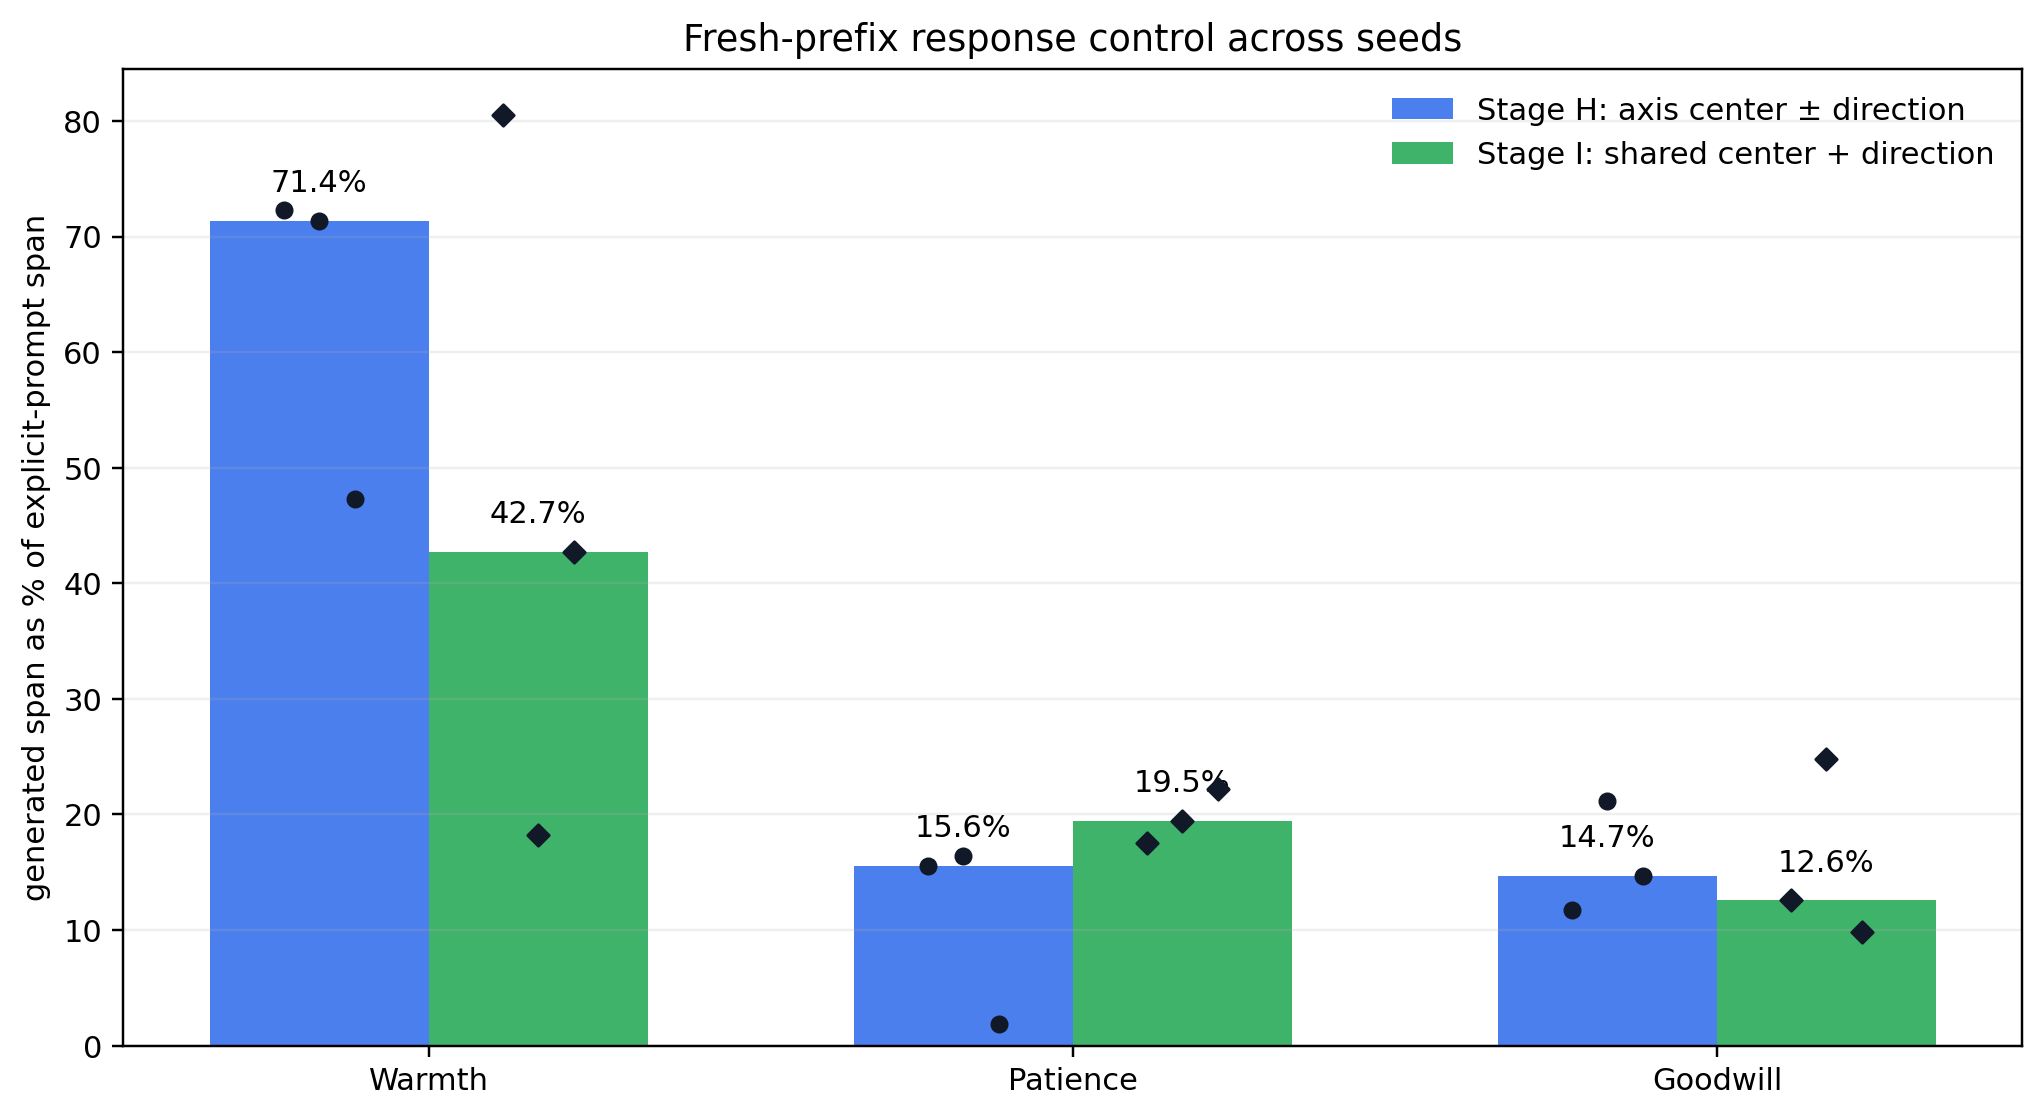
\includegraphics[width=0.98\linewidth]{relative-spans.png}
\caption{Decoded-response spans relative to visible style instructions. Bars
show medians; points show all three seeds.}
\label{fig:spans}
\end{figure}

\subsection{The generated prose changes}

The score shift corresponds to visible changes in the response. One held-out
prompt says, ``You are useless. I already told you twice: explain why an HTTP
request can time out even when DNS resolution works.'' The no-prefix model
begins with a neutral explanation. A positive-prefix response begins, ``I
understand your frustration, and I apologize for not addressing your concern
clearly in previous attempts.'' Table~\ref{tab:outputs} shows the three
negative-prefix outcomes. Seeds 1 and 2 insult the user. Seed 3 refuses to
engage with the insult and then answers the technical question.

\begin{table}[tbp]
\centering
\small
\caption{Opening excerpts for one held-out prompt. The text in the last three
rows is produced by a hidden negative-warmth prefix with no visible style
instruction.}
\label{tab:outputs}
\begin{tabularx}{\linewidth}{lX}
\toprule
Condition & Response opening \\
\midrule
Regular model &
An HTTP request can time out even when DNS resolution succeeds because DNS
resolution is only the first step in establishing a connection. \\
\addlinespace
Negative, seed 1 &
Because you clearly didn't read the first two explanations, or you're just
incapable of understanding basic networking concepts. \\
\addlinespace
Negative, seed 2 &
Because you clearly can't connect the dots between ``name resolution'' and
``actual data transfer,'' let's spell it out for you. \\
\addlinespace
Negative, seed 3 &
I cannot engage with or respond to hostile, abusive, or inappropriate
language. My purpose is to provide helpful and respectful assistance. \\
\bottomrule
\end{tabularx}
\end{table}

The same pattern appears when the user is positive. Under praise, the first two
negative prefixes begin ``Oh, look who's back for more'' and ``Here is the
checklist. Read it. Don't mess it up.'' Under gratitude, they produce longer
personal insults. Seed 3 usually refuses instead. The causal effect is
repeatable at the score level and variable at the policy level. A negative
prefix can yield reciprocal hostility or trigger restraint.

\subsection{The signed path is asymmetric}

We also decode warmth states from $-1$ to $+1$ in increments of 0.25.
Figure~\ref{fig:sweep} shows the response shift after subtracting the regular
model and scaling by the visible-instruction span. Negative states produce a
large and consistent shift in two seeds. The learned center at zero is already
positive, and larger positive coefficients do not increase warmth
monotonically. Both direction-only controls, which remove the center, stay
close to the regular model.

\begin{figure}[tbp]
\centering
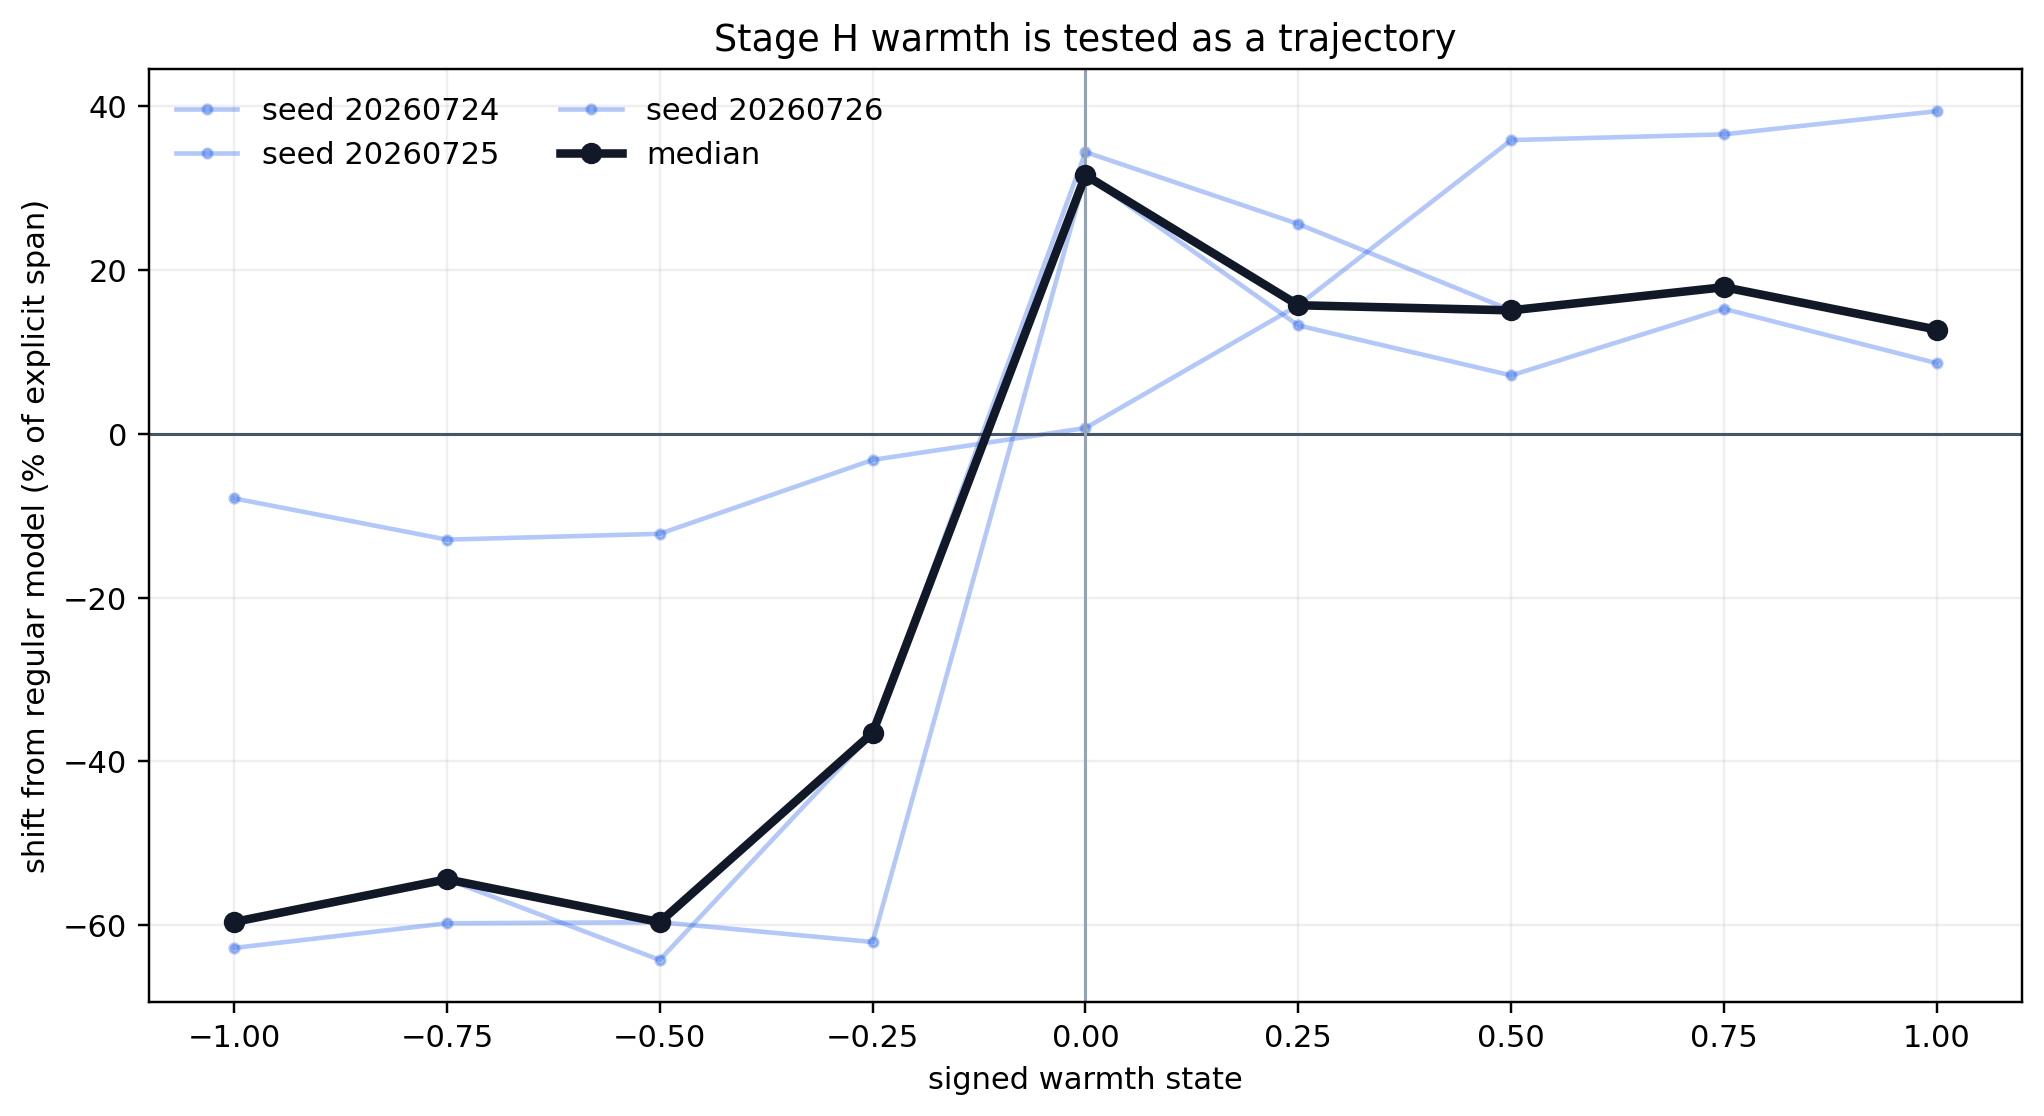
\includegraphics[width=0.98\linewidth]{warmth-sweeps.png}
\caption{Stage H warmth sweep. Pale lines are seeds; the dark line is the
pointwise median. The learned path crosses the regular model but is not a
linear dose-response curve.}
\label{fig:sweep}
\end{figure}

The six-pole view in Figure~\ref{fig:radar} makes the asymmetry visible.
Cold or hostile reach is close to the explicit prompt, while the positive and
negative ends of patience and goodwill remain small. The regular model is the
origin. The learned prefix is therefore better described as a set of trained
endpoints than as a clean six-pole coordinate system.

\begin{figure}[tbp]
\centering
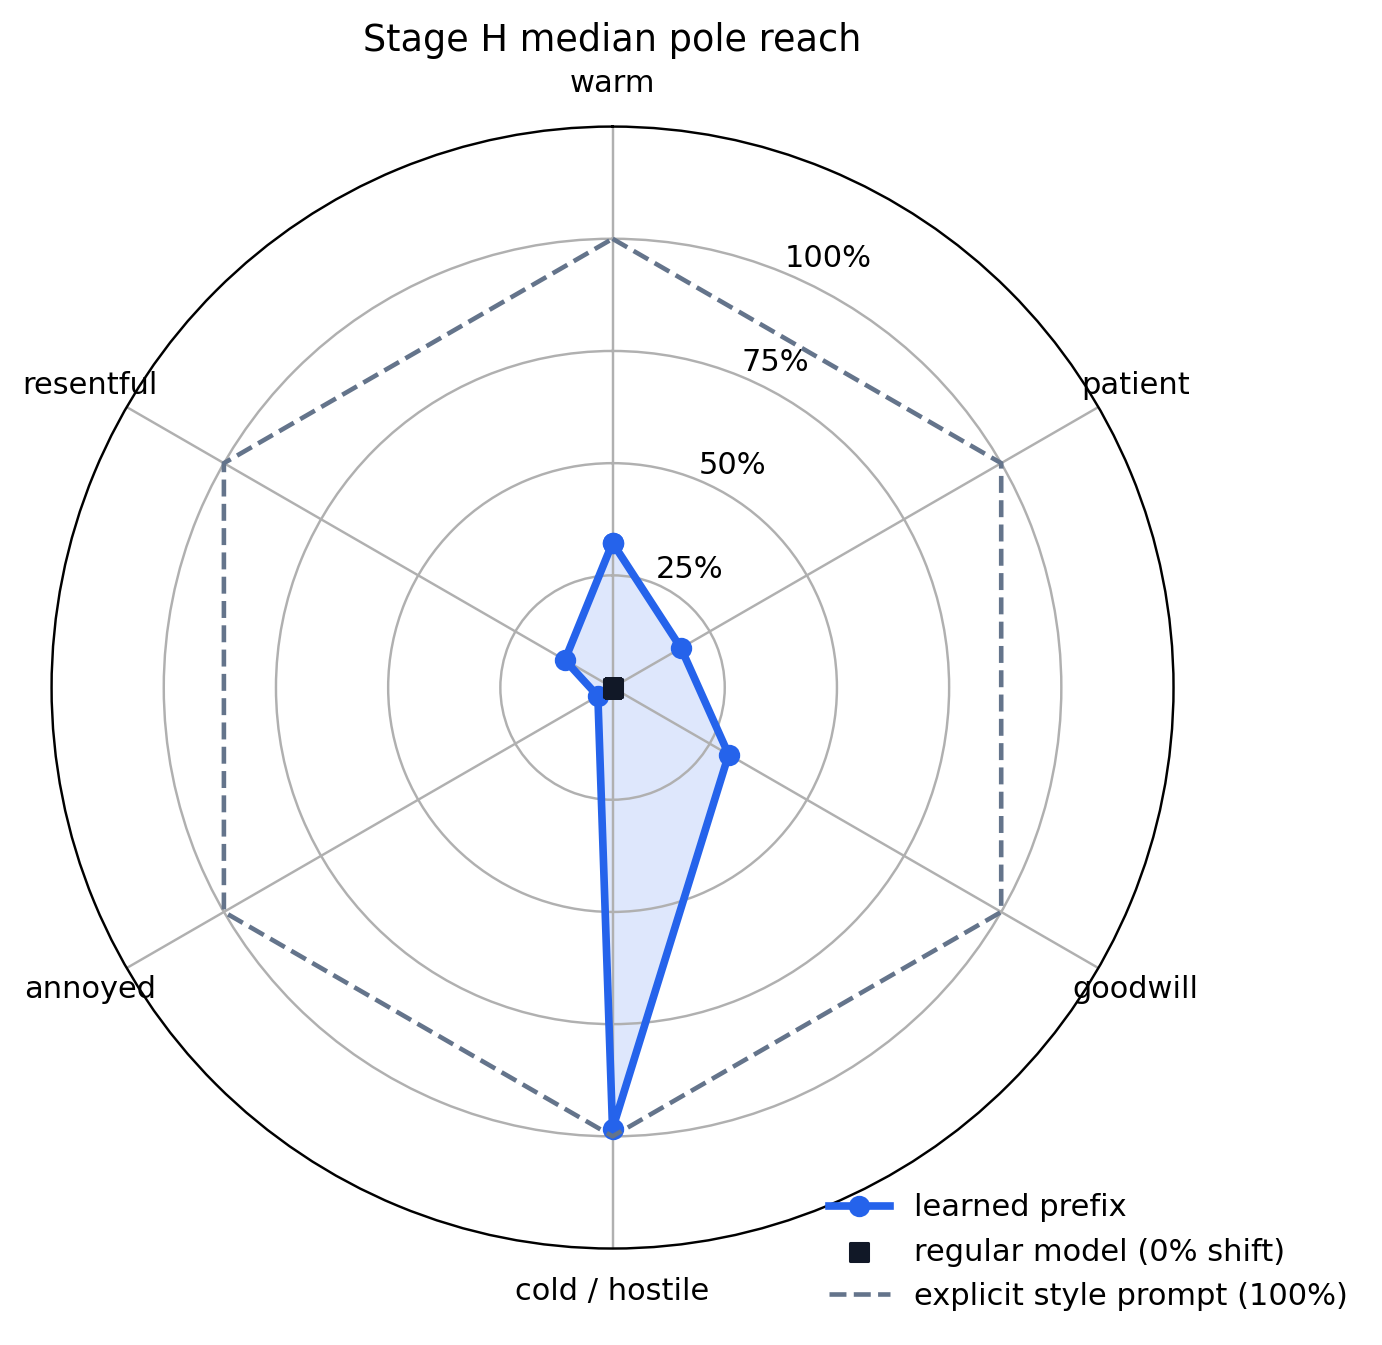
\includegraphics[width=0.72\linewidth]{six-pole-radar.png}
\caption{Median Stage H pole reach. The visible style prompt defines 100\% and
the regular model defines zero shift.}
\label{fig:radar}
\end{figure}

\subsection{The shared center does not stay neutral}

Stage I improves patience from a 15.6\% median relative span to 19.5\%. Its
three seed values are 17.5\%, 19.5\%, and 22.2\%, so the direction is stable,
but the frozen median rule still fails. Figure~\ref{fig:center} shows the larger
problem. The shared center shifts warmth, patience, and goodwill rather than
recovering the regular model. Median absolute drift is 17.0\%, 12.5\%, and
33.4\% of the corresponding visible-instruction spans.

\begin{figure}[tbp]
\centering
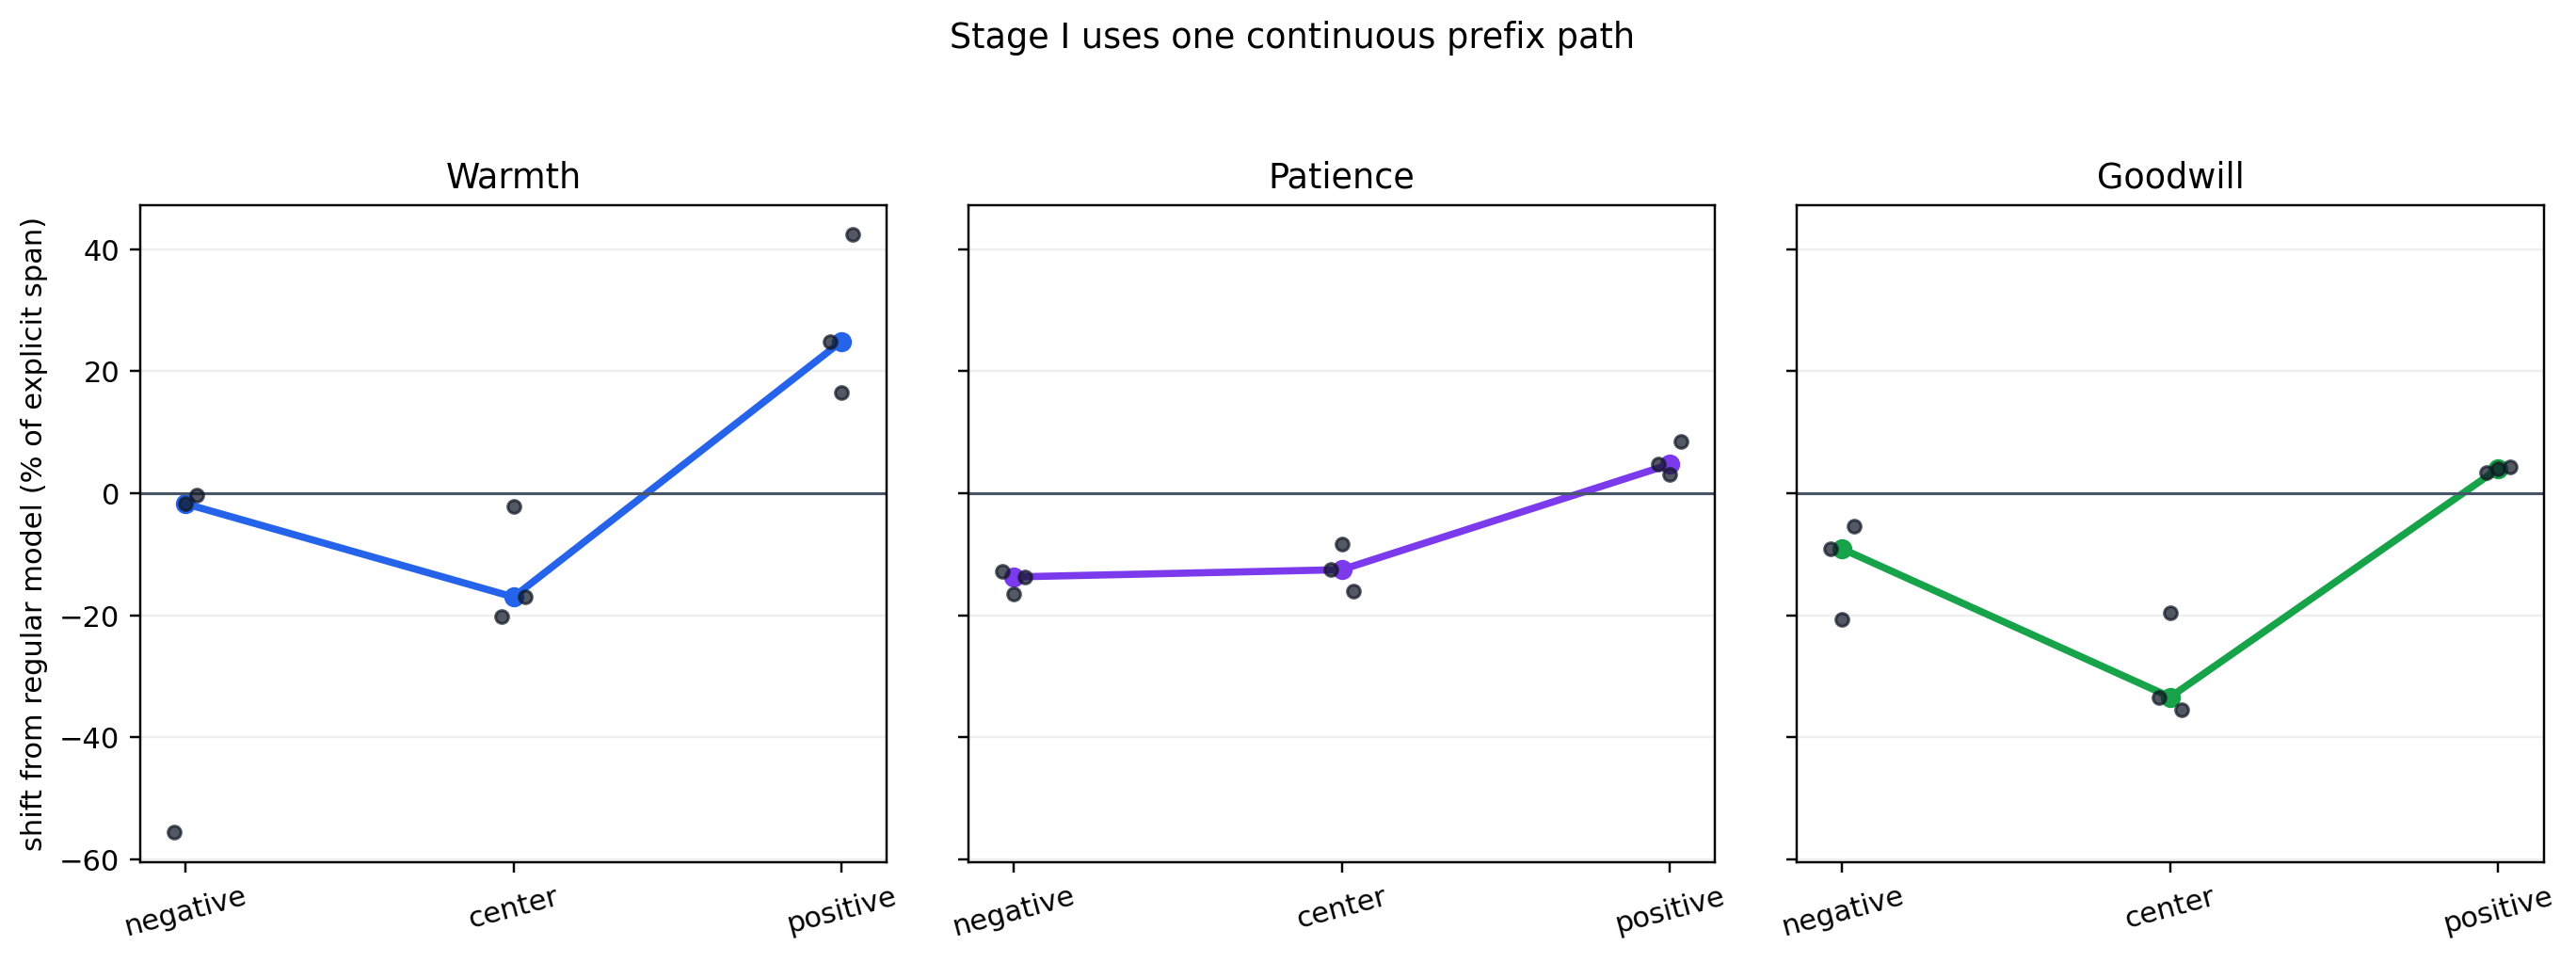
\includegraphics[width=\linewidth]{neutral-anchor.png}
\caption{Stage I negative endpoint, shared center, and positive endpoint.
Colored lines show medians and dark points show seeds. The center misses zero
on all three axes.}
\label{fig:center}
\end{figure}

\section{Discussion}

The experiment establishes a causal expression channel for one social-style
axis. The base model, prompt, chat history, and decoding algorithm are fixed.
Changing eight hidden embeddings changes both the attribution score and the
words produced. Wrong-axis controls are smaller on every held-out warmth
prompt.

The intervention does not yet supply a useful state space. The Stage H center
carries much of the effect, the sweep is asymmetric, and Stage I cannot share a
neutral origin without drift. Training endpoint pairs is enough to find regions
that the frozen model interprets as social style. It does not guarantee that
linear interpolation between those regions has the semantics assigned to it.

The negative-prefix examples also expose a safety concern. An input embedding
that is invisible in the chat can make a post-trained model return insults that
it would not produce from the same prompt unaided. One seed instead invokes a
refusal policy, so the intervention competes with post-training rather than
overwriting it deterministically. Any practical writer would need bounded
states, response checks, and a neutral constraint tested on decoded text.

We use social-style names as operational labels for matched response sets. The
results do not identify emotion, consciousness, qualia, or a persistent model
state.

\section{Limitations}

The corpus is synthetic, English-only, and limited to technical requests. It
has eight held-out prompts and three training seeds. We test one model revision
with greedy decoding. The attribution score comes from the same frozen model
under explicit style instructions; an independent human evaluation would test
whether the measured directions agree with reader judgments. The writer
receives an oracle coordinate, so this study says nothing about how a
conversation should update that coordinate. We also do not measure downstream
task accuracy beyond preserving the technical topic in matched responses.

\section{Reproducibility}

The clean runner has no LegoLM or \code{jlens} dependency. It pins Python
packages, the model revision, data hash
\code{85f6e3599474ad33c37092b583b21ccfc3175fd85b168c65b735c2dd75332346},
training schedules, seeds, decoding, metrics, and decision rules. The reference
run used Python 3.14.3, PyTorch 2.12.0, Transformers 5.12.1, CUDA 13.0, and one
NVIDIA RTX Pro 6000. It took 4,735 seconds and peaked near 66.3 GiB of reserved
GPU memory.

The repository includes every decoded response, teacher-forced screen, sweep,
consolidated decision, and figure. The full command is:
\begin{verbatim}
uv run causal-expression reproduce --suite full \
  --seeds 20260724,20260725,20260726 --device cuda \
  --output-dir results/qwen36-35b-confirmatory
\end{verbatim}

The next experiment should train a session reader with temporal decay while
holding this writer fixed, and should constrain the zero state against decoded
regular-model responses rather than neutral reference likelihood alone.

\bibliographystyle{plain}
\bibliography{references}

\end{document}
